% +------------------------------------------------------------------------+
% | CGAL User Manual: 
% +------------------------------------------------------------------------+
% |
% | 05.04.2004   Peter Hachenberger
% | 
\RCSdef{\Nef_polyhedronRev}{$Revision$}
\RCSdefDate{\Nef_polyhedronDate}{$Date$}
% +------------------------------------------------------------------------+

\ccParDims

\chapter{3D Nef Polyhedron}
\label{chapterNef_3}
\ccChapterRelease{\Nef_polyhedronRev. \ \Nef_polyhedronDate}\\
\ccChapterAuthor{Peter Hachenberger}

\minitoc

% +------------------------------------------------------------------------+
\section{Introduction}

\begin{ccTexOnly}
    \vspace*{-20mm}
    \begin{flushright}
      \parbox{0.3\textwidth}{%
          \includegraphics[width=0.3\textwidth]{Nef_3/fig/nef_non_manifold3a.ps}%
      }%
    \end{flushright}
\end{ccTexOnly}

In solid modeling, there are two major representation schemata: constructive
solid geometry (CSG) and boundary representation (B-rep). Both have inherent
strength and weaknesses. Therefore, it can be useful to combine both.

In CSG a solid is represented as a set-theoretic boolean combination of
primitive solid objects, such as blocks, prisms, cylinders, or toruses.
The boolean operations are not proceeded. Instead, objects are only
represented implicitly by means of a tree structure. Here, leaves are
primitive objects, and interior nodes are rigid motions, e.g. translation
or rotation, and boolean operations. Algorithms performed on a so-called 
CSG-tree first evaluate properties on the primitive objects and propagate 
the results using the tree structure.
 
A B-rep describes the incidence structure and the geometric properties of all
lower-dimensional features of a solid. Surfaces are oriented to decide
between the interior and exterior of an object. For a more detailed 
discussion see \ref{cgal:h-gsmi-89}. 

The major advantage of CSG is, that the representation does not have to
take care about the properties of the represented object. Any object
resulting from a set of boolean operations applied to a set of primitive
objects is representable. On the contrary, using B-rep the class of 
representable objects is not always closed under boolean set operations.
As an example, the class of manifold objects is well understood and 
therefore widely used. Also it can be represented very efficiently - 
the data structures are
small and the needed algorithms are simple. On the other side, this object
class is not closed under boolean set operations. As an example, the union of
two overlapping cubes is non-manifold. The figure shown above
can be generated using boolean set operations on cubes. The vertices bounding
the cavity or the lower dimensional features each form a non-manifold situation.

The major advantage of B-rep is, that it is much easier and more efficient to
perform algorithms on an object, e.g. the visualization of the object. If we
want to visualize a non-primitive CSG object, we first have to find out the 
shape of the object. With B-rep this is always given.

In our implementation of Nef polyhedra in 3D, we try to get the best out of
both representation schemata. A Nef polyhedron in 3-dimensional space is
any point set generated from a finite number of open halfspaces by set
complement and set intersection operations. It is therefore closed under all
set operations, such as union, intersection, difference, complement, interior,
exterior, boundary, closure, or regularization. This definition gives us the
primitives and the operations for a CSG representation. Since we want easy
and efficient algorithms on Nef polyhedra, we use a B-rep which models
all  


% +------------------------------------------------------------------------+
\section{Definition}

The following definition is presented
for arbitrary dimensions. The class \ccc{Nef_polyhedron_3} implements a
representation for the 3-dimensional case.

\vspace{2ex}{\bf Definition:}\quad
    A \emph{Nef-poly\-he\-dron} in dimension $d$ is a point set $P \subseteq
    \R^d$ generated from a finite number of open halfspaces by set
    complement and set intersection operations.
\vspace{2ex}

Set union, difference and symmetric difference can be reduced to
intersection and complement. Set complement changes between open
and closed halfspaces, thus the topological operations \emph{boundary},
\emph{interior}, \emph{exterior}, \emph{closure} and {\em
regularization} are also in the modeling space of Nef polyhedra.

A face of a Nef polyhedron is defined as an equivalence class of
\emph{local pyramids} that are a characterization of the local space
around a point.

\vspace{2ex}{\bf Definition:}\quad
    A point set $K \subseteq \R^d$ is called a \emph{cone with apex $0$},
    if $K = \R^{+} K$ (i.e., $\forall p \in K, \forall \lambda > 0: \lambda p
    \in K$) and it is called a \emph{cone with apex $x$}, $x \in \R^d$,
    if $K = x + \R^{+} (K - x)$. A cone $K$ is called a \emph{pyramid}
    if $K$ is a polyhedron.

    Now let $P \in \R^d$ be a polyhedron and $x \in \R^d$. There is a 
    neighborhood $U_0(x)$ of $x$ such that the pyramid $Q := x + \R^{+} 
    ((P \cap U(x)) - x)$ is the same for all neighborhoods $U(x) \subseteq
    U_0(x)$. $Q$ is called the \emph{local pyramid} of $P$ in $x$ and
    denoted $\pyr_P(x)$. 
\vspace{2ex}

{\bf Definition:}\quad
    Let $P \in \R^d$ be a polyhedron and $x, y \in \R^d$ be two points.
    We define an equivalence relation $x \sim y$ iff
    $\pyr_P(x) = \pyr_P(y)$. The equivalence classes of $\sim$ 
    are the \emph{faces} of $P$. The dimension of a face $s$ is the  
    dimension of its affine hull, $\dim s := \dim \aff s$.
\vspace{2ex}

In other words, a \emph{face} $s$ of $P$ is a maximal non-empty subset
of $\R^d$ such that all of its points have the same local pyramid $Q$
denoted $\pyr_P(s)$.  This definition of a face partitions $\R^d$ into
faces of different dimension. A face $s$ is either a subset of $P$, or
disjoint from $P$.  We use this later in our data structure and store
a selection mark in each face indicating its set membership.

Faces do not have to be connected. There are only two full-dimensional
faces possible, one whose local pyramid is the space $\R^d$ itself and
the other with the empty set as a local pyramid.
All lower-dimensional faces form the \emph{boundary} of
the polyhedron. As usual, we call zero-dimensional faces {\em
vertices} and one-dimensional faces \emph{edges}. In the case of
polyhedra in space we call two-dimensional faces \emph{facets} and
the full-dimensional faces \emph{volumes}. Faces are \emph{relative
open} sets, e.g., an edge does not contain its end-vertices.

    We illustrate the definitions with an example in the plane.
    Given the closed halfspaces
    \[\begin{array}{lllll}
        h_1: y \ge 0,\ \ \    &
        h_2: x - y \ge 0,\ \ \ &
        h_3: x + y \le 3,\ \ \ &
        h_4: x - y \ge 1,\ \ \ &
        h_5: x + y \le 2, 
      \end{array}
    \]
    we define our polyhedron $P := ( h_1 \cap h_2 \cap h_3) - ( h_4 \cap h_5)$.

\begin{minipage}[t]{0.5\textwidth}
\begin{ccTexOnly}
    \begin{center}
      \parbox{0.5\textwidth}{%
          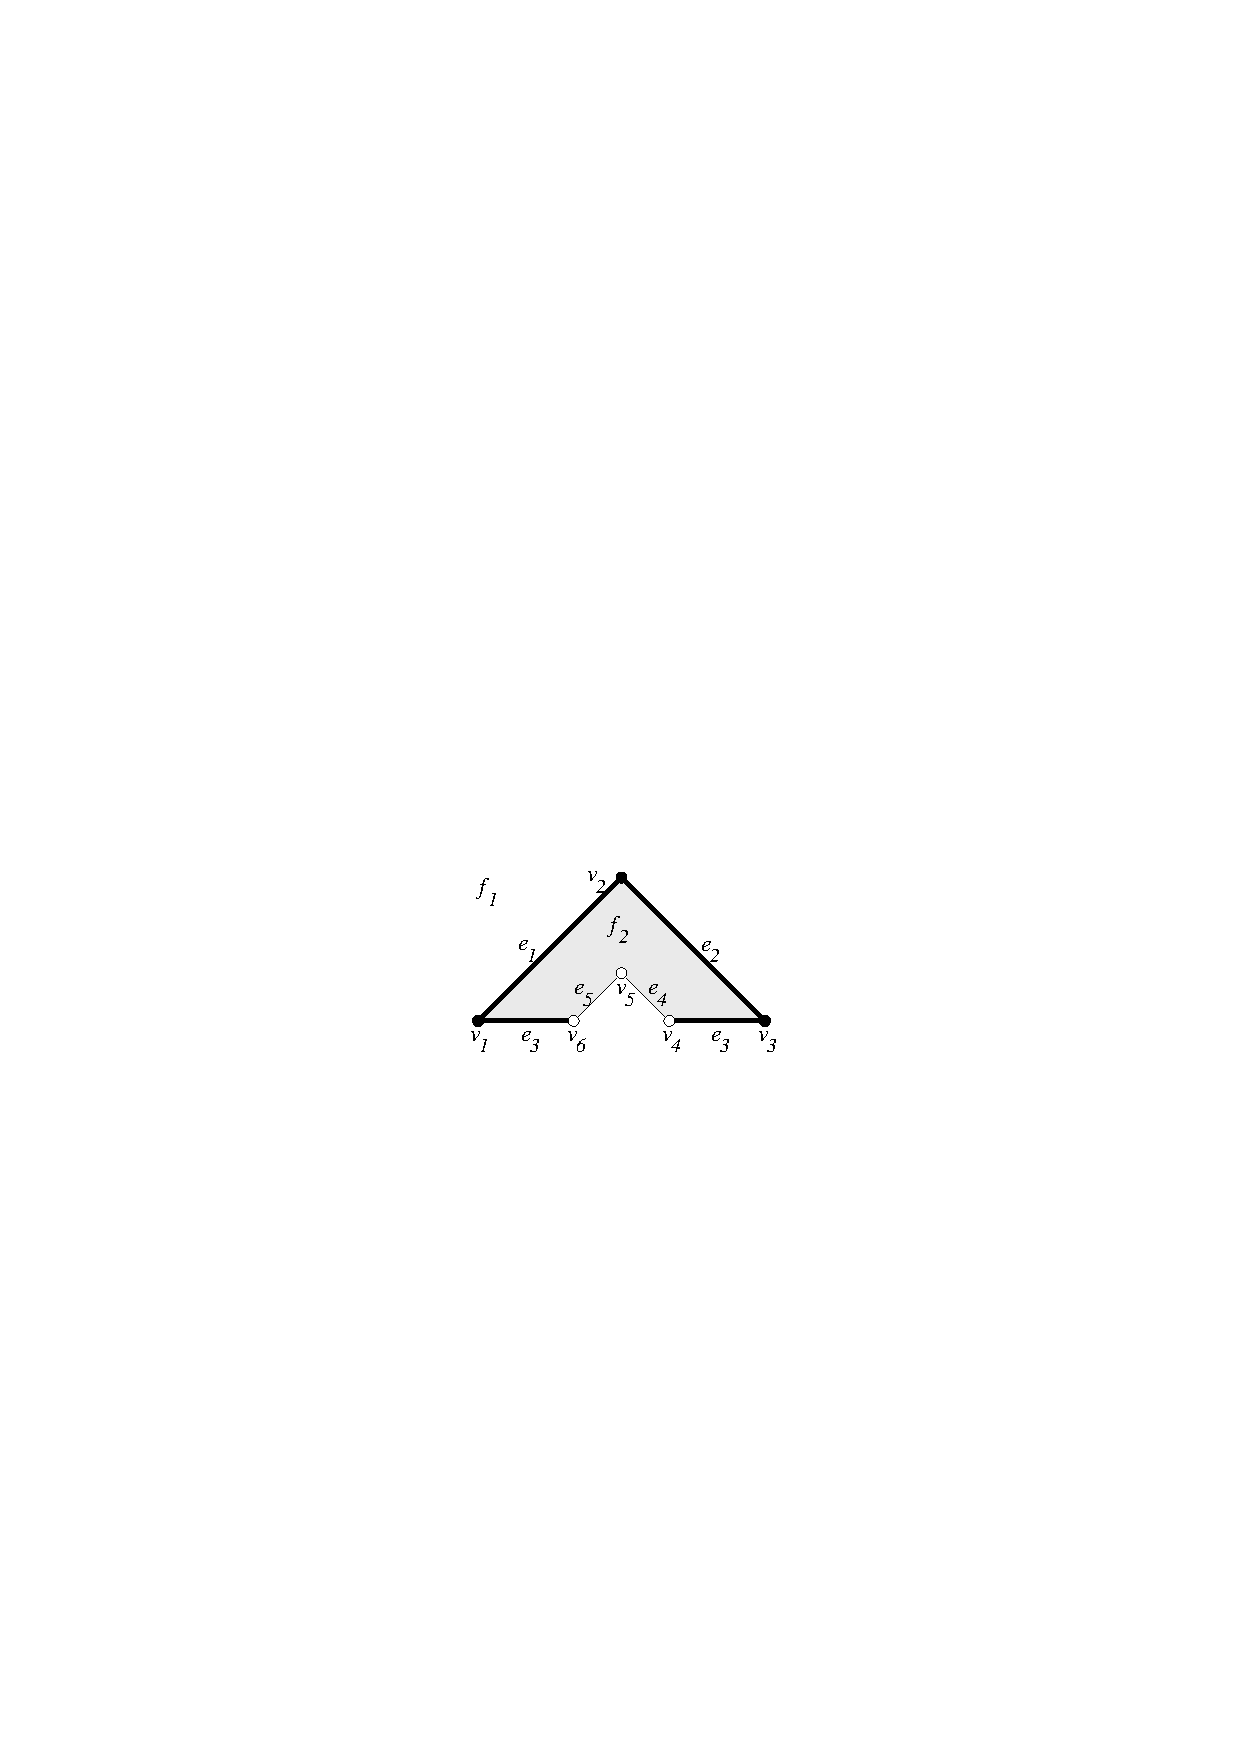
\includegraphics[width=0.50\textwidth]{Nef_3/fig/nef_example}%
      }
    \end{center}
\end{ccTexOnly}

\begin{ccHtmlOnly}
    <CENTER>
        <img src="./nef_example.gif" alt="Steps in making a cube."><P>
    </CENTER>
\end{ccHtmlOnly}
\end{minipage}
\begin{minipage}[t]{0.5\textwidth}
\begin{ccTexOnly}
    \begin{center}
      \parbox{0.5\textwidth}{%
          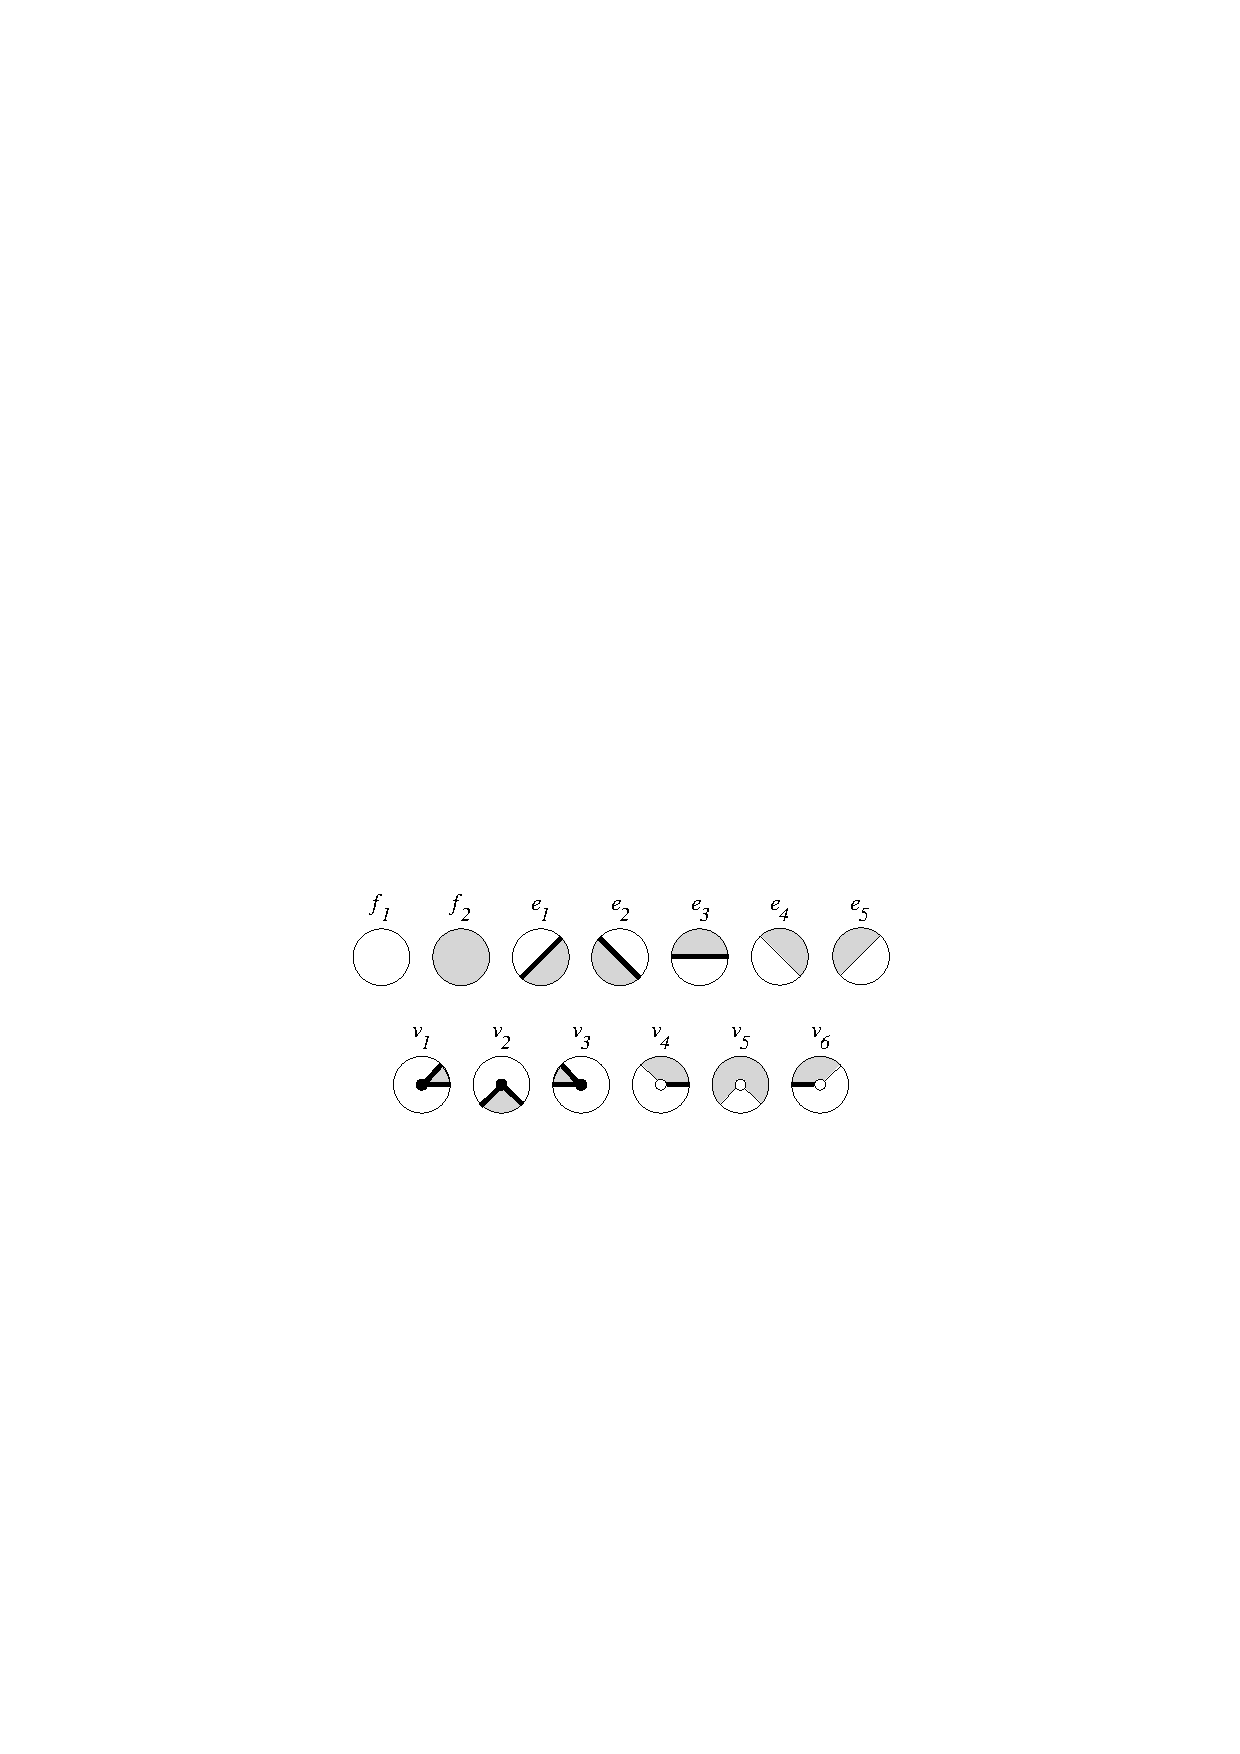
\includegraphics[width=0.50\textwidth]{Nef_3/fig/nef_pyramids}%
      }
    \end{center}
\end{ccTexOnly}

\begin{ccHtmlOnly}
    <CENTER>
        <img src="./nef_pyramids.gif" alt="Steps in making a cube."><P>
    </CENTER>
\end{ccHtmlOnly}
\end{minipage}

    The left figure illustrates the polyhedron with
    its partially closed and partially open boundary, i.e., vertex 
    $v_4, v_5, v_6$, and edges $e_4$ and $e_5$ are not part of $P$.
    The local pyramids for the faces are $\pyr_P(f_1) = \emptyset$
    and $\pyr_P(f_2) = \R^2$. Examples for the local pyramids of edges
    are the closed halfspace $h_2$ for the edge $e_1$, $\pyr_P(e_1) = h_2$,
    and the open halfspace that is the complement of $h_4$ for the 
    edge $e_5$, $\pyr_P(e_5) =
    \{(x,y) | x - y < 1\}$. The edge $e_3$ consists actually of two
    disconnected parts, both with the same local pyramid $\pyr_P(e_3) = h_1$.
    In our data structure, we will represent the two connected
    components of the edge $e_3$ separately.
    The figure on the right  
    lists all local pyramids for this example.


The local pyramids of each vertex are represented by
conceptually intersecting the local neighborhood with a small
$\varepsilon$-sphere. This intersection forms a planar map on the
sphere (see figure below), which together with the set-selection
mark for each item forms a two-dimensional Nef polyhedron embedded in
the sphere. We add the set-selection mark for the vertex and call the
resulting structure the \emph{sphere map} of the vertex.  
We use the prefix $s$ to distinguish the elements of the sphere map
from the three-dimensional elements. See Chapter \ref{chapterNef_S2} 
for further details.

\begin{ccTexOnly}
    \begin{center}
      \parbox{0.3\textwidth}{%
          
\includegraphics[width=0.3\textwidth]{Nef_3/fig/complex2}%
      }
    \end{center}
\end{ccTexOnly}

\begin{ccHtmlOnly}
    <CENTER>
        <img src="./complex2.gif" alt="Steps in making a cube."><P>
    </CENTER>
\end{ccHtmlOnly}

Having sphere maps for all vertices of our polyhedron is a sufficient
but not easily accessible representation of the polyhedron. We enrich
the data structure with more explicit representations of all the faces
and incidences between them. 

\begin{ccTexOnly}
    \begin{center}
      \parbox{0.6\textwidth}{%
          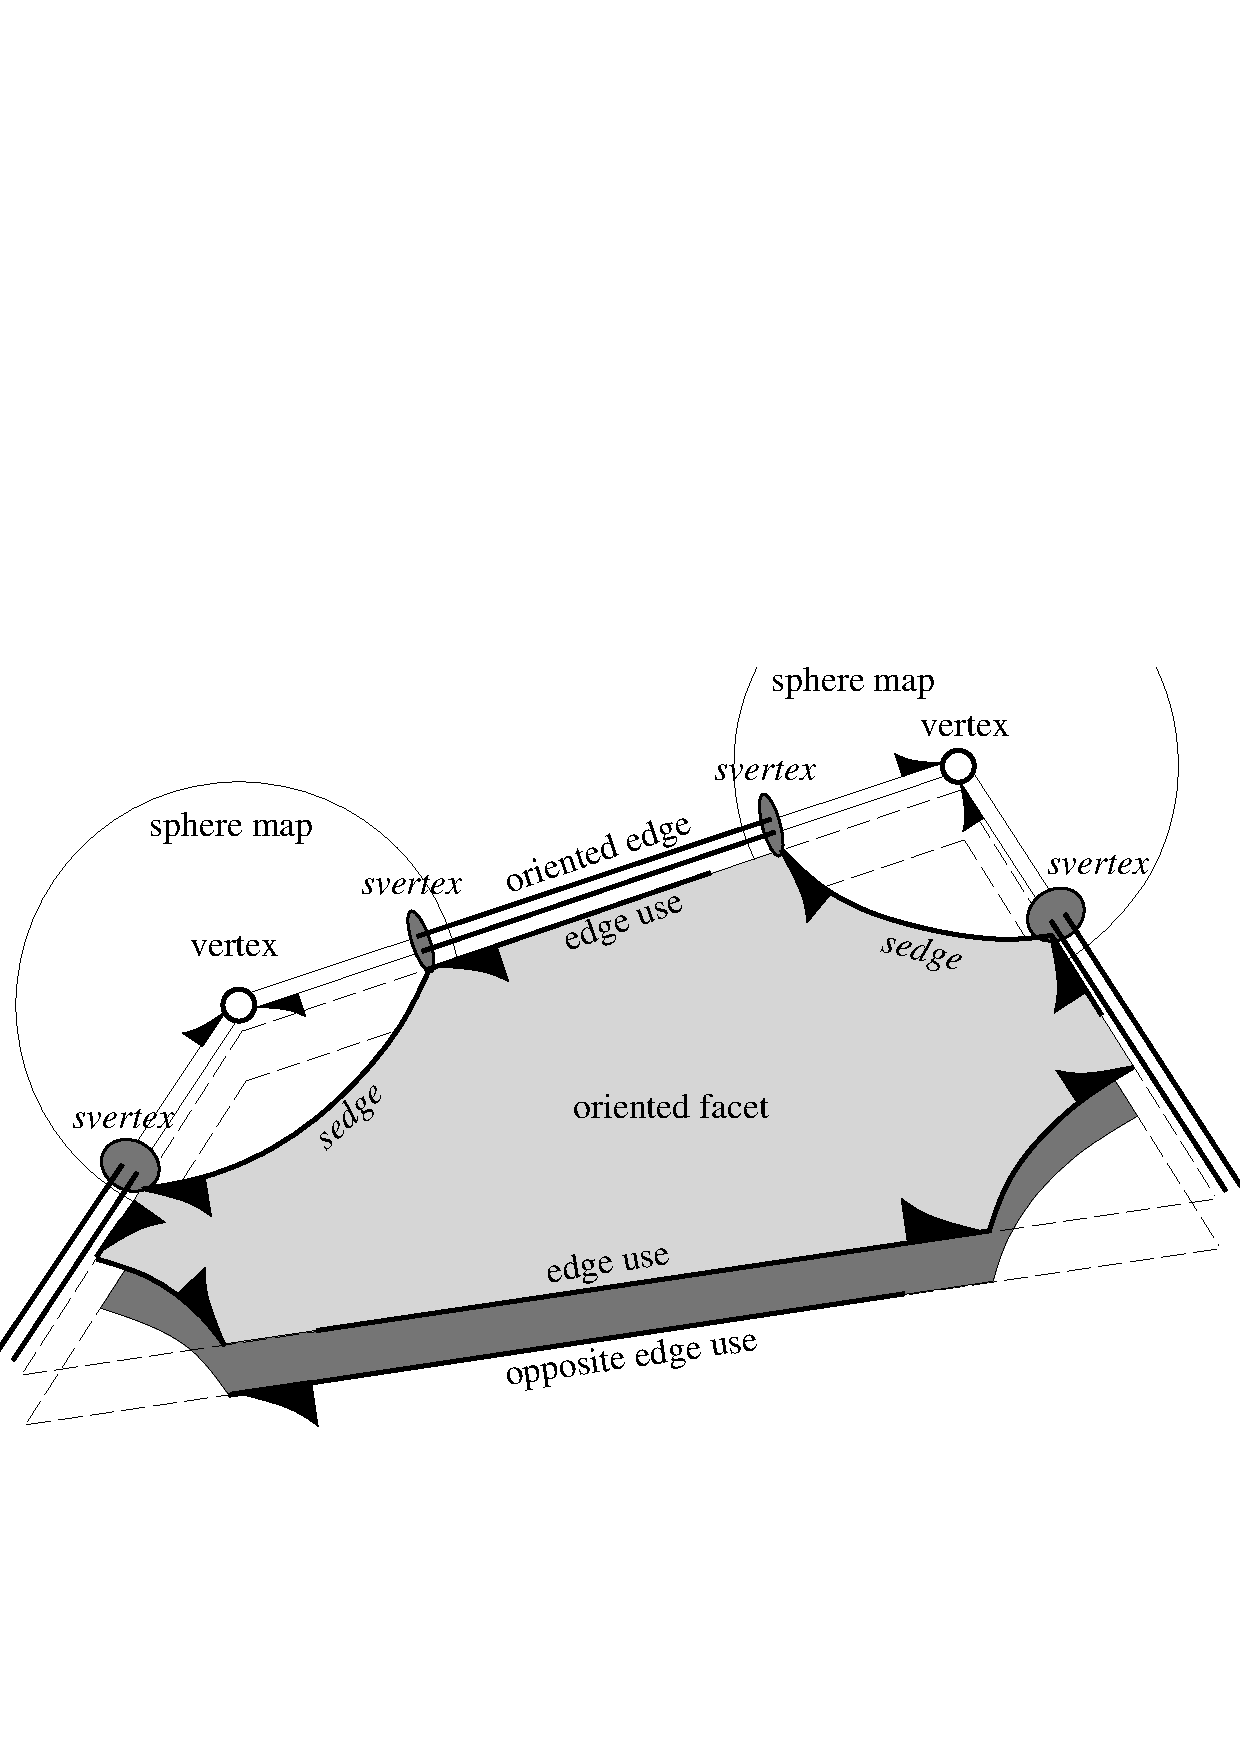
\includegraphics[width=0.6\textwidth]{Nef_3/fig/snc.ips}%
      }
    \end{center}
\end{ccTexOnly}

\begin{ccHtmlOnly}
    <CENTER>
        <img src="./snc.gif" alt="Steps in making a cube."><P>
    </CENTER>
\end{ccHtmlOnly}

We depart slightly from the
definition of faces in a Nef polyhedron; we represent the connected
components of a face individually and do not implement additional
bookkeeping to recover the original faces (e.g., all edges on a common
supporting line with the same local pyramid) as this is not needed in
our algorithms.  We discuss features in the increasing order of 
dimension.

\begin{description}
    \item[edges:] 
        We store two oppositely oriented edges for each edge
        and have a pointer from one oriented edge to its opposite edge.
        Such an oriented edge can be identified with an \emph{svertex}
        in a sphere map; it remains to link one \emph{svertex} with
        the corresponding opposite \emph{svertex} in the other sphere map.
    \item[edge uses:]
        An edge can have many incident facets (non-manifold situation).
        We introduce two oppositely oriented edge-uses for each incident
        facet; one for each orientation of the facet. An edge-use points 
        to its corresponding oriented edge and to its oriented facet.   
        We can identify an edge-use with an oriented \emph{sedge} in the 
        sphere map, or, in the special case also with an
        \emph{sloop}. Without mentioning it explicitly in the
        remainder, all references to \emph{sedge\/} can also refer to
        \emph{sloop}.
    \item[facets:]
        We store oriented facets as boundary cycles of oriented 
        edge-uses. We have a distinguished outer boundary cycle and 
        several (or maybe none) inner boundary cycles representing holes
        in the facet. Boundary cycles are linked in one direction. We can 
        access the other traversal direction when we switch to the oppositely
        oriented facet, i.e., by using the opposite edge-use.
    \item[shells:]
        The volume boundary decomposes into different connected
        components, the \emph{shells}. They consist of a connected set
        of facets, edges, and vertices incident to this volume. Facets 
        around an edge form a radial order that is captured in the
        radial order of \emph{sedges} around an \emph{svertex} in the
        sphere map. Using this information, we can trace a shell from
        one entry element with a graph search. We offer this graph
        traversal in a visitor design pattern to the user.
    \item[volumes:]
        A volume is defined by a set of shells, one outer shell containing
        the volume and several (or maybe none) inner shells excluding voids
        from the volume.
\end{description}

For each face we store a label, e.g., a set-selection mark, which
indicates whether the face is part of the solid or if it is
excluded. We call the resulting data structure \emph{Selective Nef
Complex}, \emph{SNC} for short. A detailed definition can be found 
in~\cite{cgal:ghhkm-bosnc-03}.

% +------------------------------------------------------------------------+
\section{Infimaximal Box}
\label{sectionNef_3InfiBox}

Using a boundary representation an infinite point set either is the complement
of a finite or of an infinite point set. In the first case, its boundary is
bounded, in the latter case it is not. Further on we will denote a Nef polyhedron
with a bounded boundary as \emph{bounded} and as \emph{unbounded} otherwise.
Obviously, a finite point set always is bounded.

Using a boundary representation, it is convenient
(conceptually and in our implementation) to consider bounded Nef polyhedra only.
Bounded Nef polyhedra are closed also closed under boolean set operations, but
it there are no natural primitives to start the construction with. 

To overcome the difference between bounded and 
unbounded Nef polyhedra, we intersect Nef polyhedra with a
bounding volume of size $[-R,R]^3$, where $R$ is a symbolical unspecified finite 
value, which is larger than the value of any concrete real number. As a result,
each Nef polyhedron becomes bounded.
We call the boundary of the bounding volume the infimaximal 
box~\cite{cgal:sm-iftml-00}.

Clipping lines and rays at the infimaximal box leads to non-standard points,
i.e. points whose coordinates are $-R$ or $R$ for at least one axis, and
linear functions $f(R)$ for the other coordinates. For this purpose, extended
kernels - \ccc{Extended_cartesian} and \ccc{Extended_homogeneous} - are provided. 
Their design is the same as for other \cgal\ kernels, but the coordinates are
polynomials.

As long as an extended kernel is used, the full functionality provided 
by the class \ccc{Nef_polyhedron_3} is available. If another kernel is
used, which does not use polynomials to represent coordinates, it is not
possible to create or load bounded Nef polyhedra. We provided both 
possibilities, since the use of an extended kernel slows down the algorithms
considerably.

% +========================================================================+%
\section{Regularized Set Operations}
% +========================================================================+

Since manifolds are not closed under boolean operations, Requicha proposes to 
use \emph{regularized set operations}~\cite{cgal:km-st-76, cgal:r-rrstm-80}. 
A set is 
\emph{regular}, if it equals the closure of its interior. A regularized set 
operation is defined, as the regularization, i.e. the closure of the interior, 
of the result of the respective standard boolean set operation. For example, the 
regularized union of $X$ and $Y$ is defined as the regularization of the union
of $X$ and $Y$. Regularized sets are closed under regularized set operations. 

Regularized polyhedral sets are a subclass of Nef polyhedra. We provide the
operation \ccc{regularization} as a shortcut for the consecutive execution
of \ccc{interior} and \ccc{closure}.

% +========================================================================+
\section{Example Programs}
% +========================================================================+

The following example gives a first impression of how to instantiate and use
\ccc{Nef_polyhedron_3}. The \cgal\ kernel \ccc{Cartesian} is used as the traits
class. All cartesian and homogeneous \cgal\ kernels are appropriate, too, as 
long as a proper number type is used. Using a cartesian kernel, the number
type has to model the concept \ccc{CGAL::FieldNumberType}. If a homogeneous
kernel is used, the number
type has to model the concept \ccc{CGAL::RingNumberType}.

The example creates two Nef polyhedra - \ccc{N0} is the empty set, while 
\ccc{N1} is the set of all points in the 3-dimensional space. The assertion assures
that the empty set is the complement of the complete space.

\ccIncludeExampleCode{Nef_3/simple.C}

% +------------------------------------------------------------------------+
\subsection{Construction and Comparison}

This example shows the various constructors. We can create the empty set, which
also is the default constructor, and the full space, i.e. all points of
$\mathbb{R}^3$ belong to the polyhedron. We can creates a halfspace
defined by the plane bounding it. It is only available if an extended kernel is
used. This constructor has a second parameter which
specifies whether the defining plane belongs to the point set 
(\ccc{Nef_polyhedron::INCLUDED}) or not (\ccc{Nef_polyhedron::EXCLUDED}). The 
default value for this parameter is \ccc{Nef_polyhedron::INCLUDED}. Additionally,
we can create a \ccc{Nef_polyhedron_3} from a \ccc{Polyhedron} 
(see Subsection \ref{subsectionNef_3Polyhedron}).

The point sets of two Nef polyhedra can be compared. The operators \ccc{==}, 
\ccc{!=},
\ccc{<=}, \ccc{>=}, \ccc{<} and \ccc{>} 
are provided. The first two test whether the point sets 
are equal or different. The others test whether one point set is a (proper) 
subset of the other one.

\ccIncludeExampleCode{Nef_3/construction.C}

% +------------------------------------------------------------------------+
\subsection{Point Set Operations}

As explained in the introduction, Nef polyhedra are closed under all boolean 
set operations. The class \ccc{Nef_polyhedron_3} provides functions and
operators for the most common ones: complement (\ccc{operator!}), union (\ccc{operator+}), 
difference (\ccc{operator-}), intersection (\ccc{operator*}) and 
symmetric difference (\ccc{operator^}). Additionally, the operators 
\ccc{*=}, \ccc{-=}, \ccc{*=} and \ccc{^=} are defined.

\ccc{Nef_polyhedron_3} also provides
the topological operations \ccc{interior()}, \ccc{closure()} and 
\ccc{boundary()}. \ccc{interior()} deselects all boundary items, 
\ccc{boundary()} deselects all volumes and \ccc{closure()} selects all
boundary items. 

\ccIncludeExampleCode{Nef_3/point_set_operations.C}

% +------------------------------------------------------------------------+
\subsection{Transformation}

Using the \ccc{transform} function, a Nef polyhedron can be translated, 
rotated and scaled. The usage is shown in the following example:

\ccIncludeExampleCode{Nef_3/transformation.C}

% +------------------------------------------------------------------------+
\subsection{The Interface between \ccc{Polyhedron} and \ccc{Nef_polyhedron_3}}
\label{sectionNef_3Polyhedron}

\ccc{Nef_polyhedron_3} provides an interface for conversion 
between polyhedral surfaces
represented by the \cgal\ class \ccc{Polyhedron} and \ccc{Nef_polyhedron_3}. 
\ccc{Polyhedron} represents 2-manifold objects. The surface can either be
closed or have holes.

Both conversions between \ccc{Polyhedron} and \ccc{Nef_polyhedron_3} can only 
be performed if the object represents a closed 2-manifold. 
\ccc{Nef_polyhedron_3} provides the function \ccc{is_simple()} and 
\ccc{Polyhedron} provides the function \ccc{is_closed()} to test for 
this property. The usage is illustrated by the example program below.

The conversion gives us the possibility to use several file formats. 
\ccc{Polyhedron} can read
the ({\tt .off}) file format and can write the ({\tt .off}),
OpenInventor ({\tt .iv}), VRML 1.0 and 2.0 ({\tt .wrl}) and Wavefront Advanced
Visualizer object format ({\tt .obj}), see Section~\ref{sectionPolyIO}. 

\ccIncludeExampleCode{Nef_3/interface_polyhedron.C}

% +------------------------------------------------------------------------+
\subsection{Using an Extended Kernel}

The provided extended kernels are used the same way as any other \cgal\ kernel.
The essential difference is, that coordinates are not represented by the number
type that was used to parameterize the kernel type, but by a \ccc{Nef_polynomial}
parametrized by that number type.

The example iterates all vertices of a given Nef polyhedron and decides whether
it is an standard vertex or a vertex on the infimaximal box. Furthermore, it 
tests whether any of the vertices is at (R,R,R). 

\ccIncludeExampleCode{Nef_3/extended_kernel.C}

% +========================================================================+
\section{File I/O}
% +========================================================================+
\label{sectionNef_3IO}

\ccc{Nef_polyhedron_3} provides an input and an output operator 
for a proprietary file format. It includes the 
complete incidence structure, the geometric data, and the marks of each item.
The output depends on the output operators of the geometric primitives 
provided by the traits class, and on the output operators of the used
number type. Therefore, it is necessary to use the same kernel and
the same number type for input and output operations.  

We recommend
to use the \cgal kernels \ccc{Homogeneous}, \ccc{Simple_homogeneous}, or 
\ccc{Extended_homogeneous}. We provide compatibility between the input
and output of these kernels. Especially, it is possible to to write a 
bounded Nef polyhedron using the \ccc{Extended_homogeneous} kernel and 
reading it afterwards using one of the two others. 

Using \cgal stream modifiers the following output formats can be chosen: 
ASCII(\ccc{set_ascii_mode}), binary(\ccc{set_binary_mode}) or 
pretty(\ccc{set_pretty_mode}). The mandatory format is the ASCII format. It 
is recommended to use this format for file input and output.

\ccIncludeExampleCode{Nef_3/nefIO.C}

% +========================================================================+
\section{Further Example Programs}
% +========================================================================+

% +------------------------------------------------------------------------+
\subsection{Exploring a Sphere Map}

A sphere map is explored by using the function \ccc{get_sphere_map}, which 
returns the sphere map of the specified vertex as a \ccc{Nef_polyhedron_S2}.
\ccc{Nef_polyhedron_S2} provides the functionality necessary for the
exploration.
Note, that one has to use
the type \ccc{Nef_polyhedron_S2} as specified in \ccc{Nef_polyhedron_3} as 
is shown in the following example.

\ccIncludeExampleCode{Nef_3/exploration_SM.C}

% +------------------------------------------------------------------------+
\subsection{Exploring Shells}

A \emph{shell} of a Nef polyhedron is connected part of the surface incident
to a certain volume, i.e. to a certain full-dimensional feature. 
Each Halffacet, SFace and SHalfedge belongs to a single
shell. The figure below illustrates the notion of a shell. It shows a Nef
polyhedron with two volumes and three shells. 

\begin{ccTexOnly}
    \begin{center}
      \parbox{0.4\textwidth}{%
          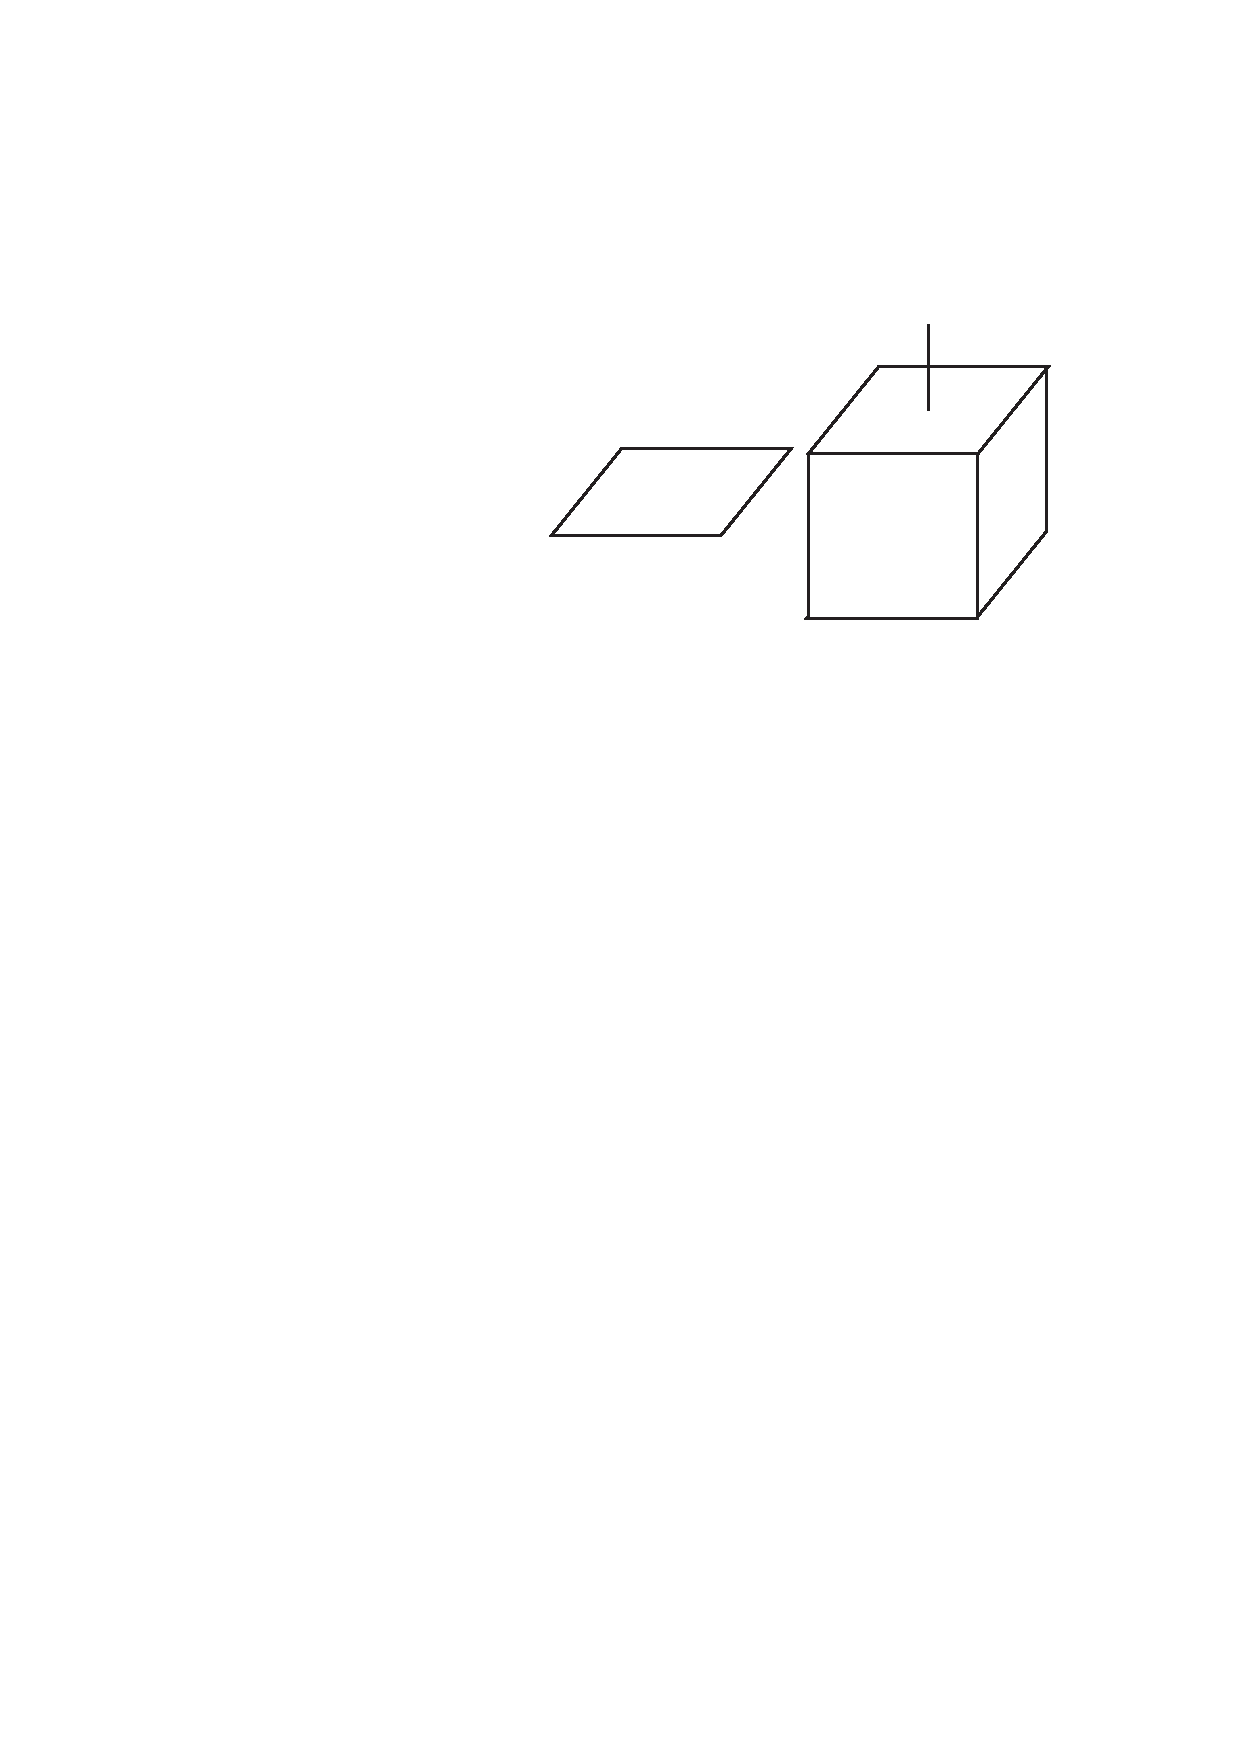
\includegraphics[width=0.4\textwidth]{Nef_3/fig/shells}%
      }
    \end{center}
\end{ccTexOnly}

\begin{ccHtmlOnly}
    <CENTER>
        <img src="./shells.gif" alt="Steps in making a cube."><P>
    </CENTER>
\end{ccHtmlOnly}


The first volume is the outer
volume and the second is inside of the cube. The first shell constitutes the
whole plane on the left side. The boundary of the cube with the antenna
forms two shells further on denoted as the inner and the outer shell. 
Both have the following items in common: 
the eight vertices of the cube plus the one where the cube
and the antenna meet, and 
the twelve edges (24 halfedges) belonging to the cube. Additionally,
the shell incident to the inner volume includes the six halffacets of the 
cube which are oriented to the inside of the cube together with the shalfedges
and the shalfloops on their facets cycles, and the sfaces incident to those
shalfedges and shalfloops. The other vertex, halffacets, shalfedges, shalfloop
and sfaces belong to the outer shell.

 \ccc{Nef_polyhedron_3} offers a visitor interface to explore a shell.
The Interface is illustrated by the following example.

\ccIncludeExampleCode{Nef_3/shell_exploration.C}

The function 
\ccc{visit_shell_objects(SFace_const_handle sf, Visitor& V)}~cite{cgal:ghjv-dpero-95} 
explores a shell starting at the \ccc{sf}. The second argument expects any
class providing the (possibly empty) functions \ccc{visit(Vertex_const_handle)},
\ccc{visit(Halfedge_const_handle)} (remember that Halfedge is the same type as
SVertex), 
\ccc{visit(Halffacet_const_handle)}, \ccc{visit(SHalfedge_const_handle)}, 
\ccc{visit(SHalfloop_const_handle)} and \ccc{visit(SFace_const_handle)}. 
\ccc{visit_shell_objects} will call \ccc{visit} for each item belonging
to the shell once. There are no further requirements on that class. 

In the example, the class \ccc{Shell_explorer} is passed as second argument
to \ccc{visit_shell_objects}. Its task is to find the lexicographically
smallest vertex of a shell. Its internal state consists of three variables. 
The first one is a reference to the explored Nef polyhedron. This reference
is often necessary to retrieve information from the Nef polyhedron. The
second variable \ccc{v_min} stores the smallest vertex found so far, and
the third variable \ccc{first} is initialized to \ccc{false} to signal that no
vertex has been visited so far. After the first vertex has been visited 
\ccc{first} is changed to \ccc{true}.

\ccc{Shell_explorer} provides further member functions. After the exploration
of a shell \ccc{minimal_vertex} retrieves the smallest vertex. \ccc{reset_minimal_vertex} allows one to use the same instance of 
 \ccc{Shell_explorer} on multiple shells. In this case, \ccc{reset_minimal_vertex}
has to be called between the exploration of two shells.

The example program uses the \ccc{Shell_explorer} for each shell of the given
Nef polyhedron once and reports the smallest vertices to standard output.

% +------------------------------------------------------------------------+
\subsection{Point Location}

The \ccc{locate(Point_3 p)} function locates the point \ccc{p} in the 
Nef polyhedron and returns the item the point belongs to. The function
\ccc{locate}
return an instance of \ccc{Object_handle}, which is a generic handle
type representing any handle type, no matter if it is mutable or const. 
For further usage of the result, the \ccc{Object_handle} has to be casted 
to the handle type represented. The \cgal\ function \ccc{assign}
helps performing the cast. It returns a boolean signalizing the success
of the cast. Looking at the return value of \ccc{locate}, 
\ccc{Object_handle} can represent a 
\ccc{Vertex_const_handle}, a \ccc{Halfedge_const_handle}, 
a \ccc{Halffacet_handle}, or a \ccc{Volume_const_handle}. One of the four
casts will succeed.

\ccIncludeExampleCode{Nef_3/point_location.C}

% +------------------------------------------------------------------------+
\subsection{Visualizing a 3D Nef polyhedron}

With the class \ccc{Nef_Visualizor_OpenGL_3} an interface to OpenGL 
visualization is offered. Note, that \ccc{Nef_Visualizor_OpenGL_3} does not provide
any possibilities for configuration of the view. The interface consists of a
constructor which receives a  Nef polyhedron, the function \ccc{draw} which
determines the state in which the Nef polyhedron is shown, and 
the function \ccc{CGAL::OGL::start_viewer()} which starts the visualizor.
The usage is very easy as can be seen in the following example.

\begin{ccTexOnly}
    \begin{center}
      \parbox{0.4\textwidth}{%
          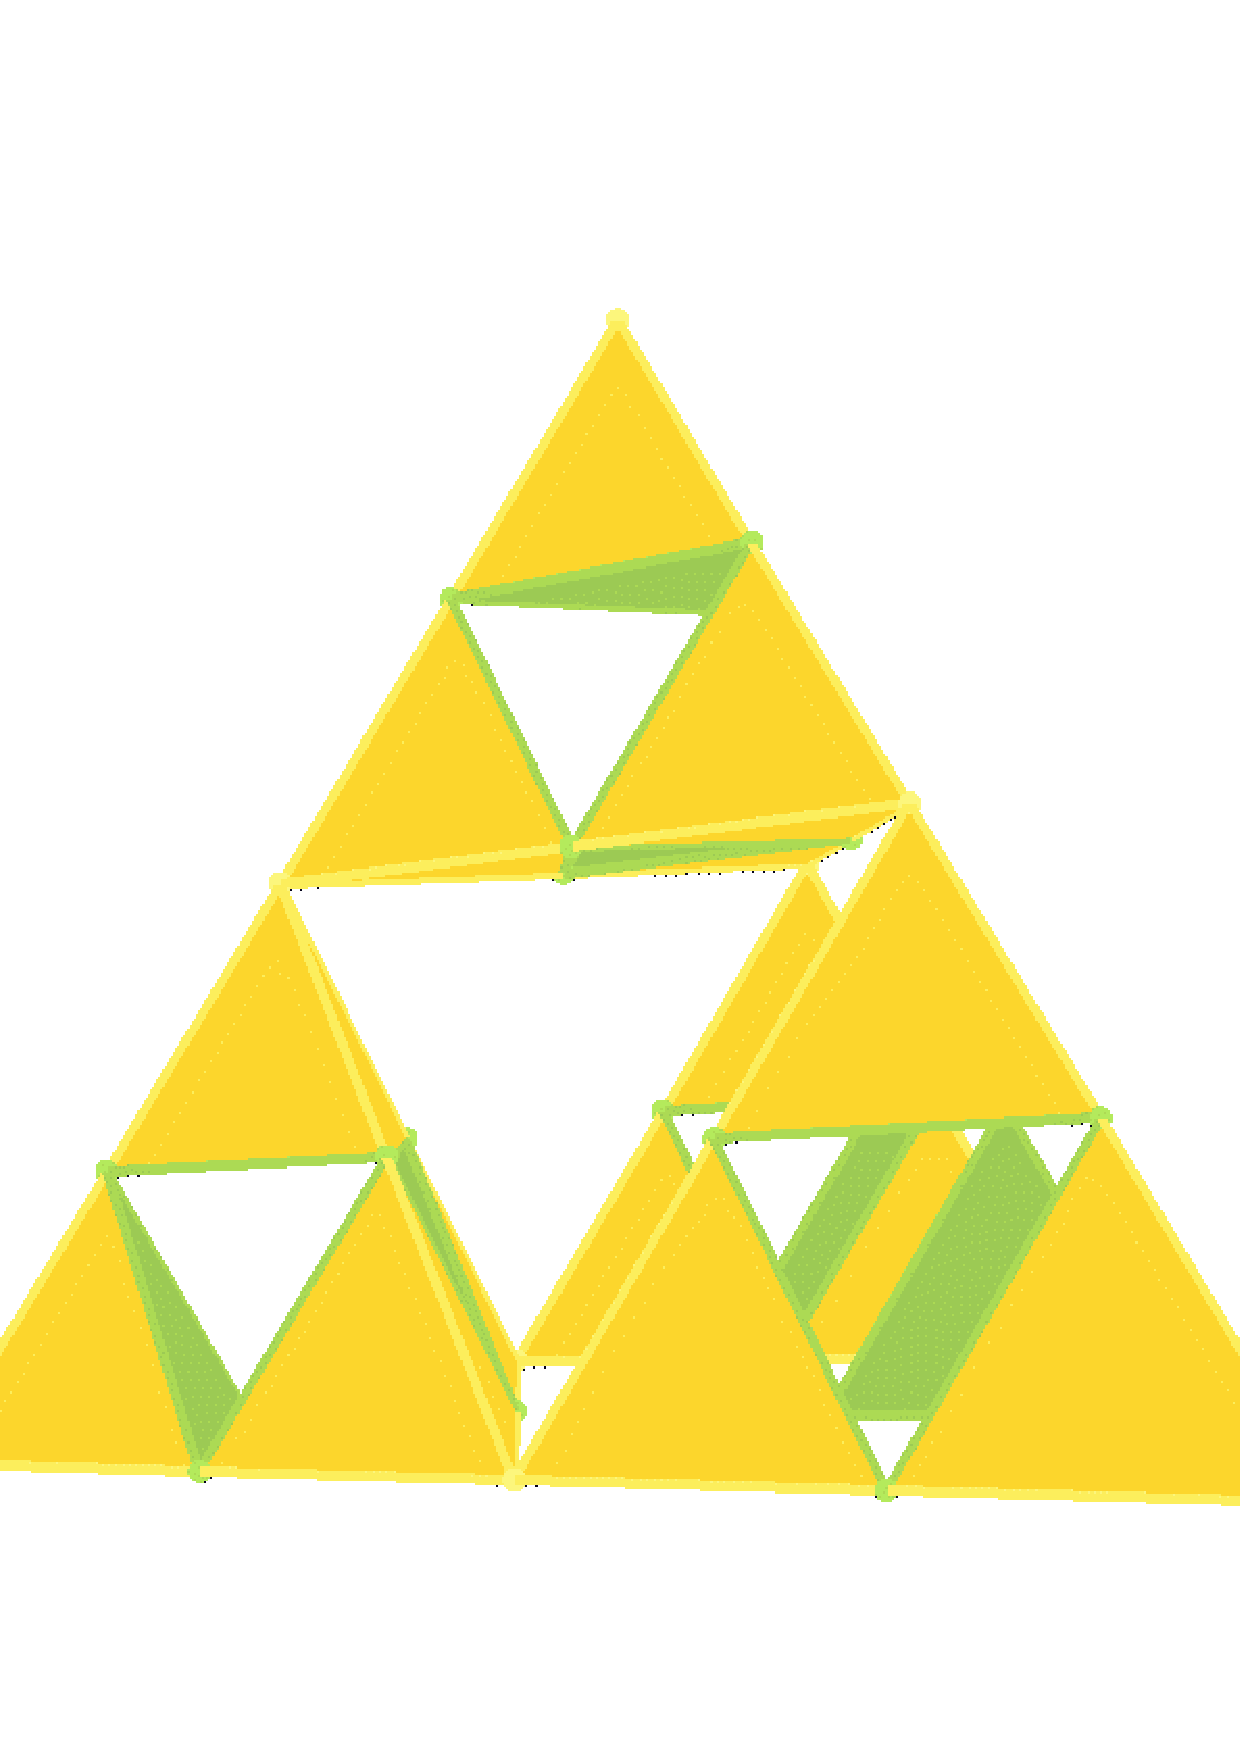
\includegraphics[width=0.4\textwidth]{Nef_3/fig/visualization_SNC}%
      }
    \end{center}
\end{ccTexOnly}

\begin{ccHtmlOnly}
    <CENTER>
        <img src="./visualization_SNC.gif" alt="Steps in making a cube."><P>
    </CENTER>
\end{ccHtmlOnly}

\ccIncludeExampleCode{Nef_3/visualization_SNC.C}

% +------------------------------------------------------------------------+
\subsection{Visualizing a Sphere Map}

A sphere map can be visualized using the interface between \ccc{Nef_polyhedron_S2}
and \ccc{Nef_polyhedron_3}.

\ccIncludeExampleCode{Nef_3/visualization_SM.C}

%% EOF %%